\حصہ{تکمل بالحصص}
تکمل بالحصص کی ترکیب سے تکمل
\begin{align}
\int f(x)g(x)\dif x
\end{align}
جس میں \عددی{f} بار بار قابل تفرق اور \عددی{g} بار بار قابل تکمل ہو کو کی سادہ روپ حاصل کی جا سکتی ہے۔ درج ذیل تکمل
\begin{align*}
\int xe^x\dif x
\end{align*}
اس قسم کا ایک تکمل ہے جہاں \عددی{f(x)=x}  دو بار تفرق کے بعد صفر ہو جاتا ہے  جبکہ \عددی{g(x)=e^x} کا تکمل بار بار لیا جا سکتا ہے۔ تکمل بالحصص کی ترکیب درج ذیل قسم کے تکمل پر بھی قابل اطلاق ہے
\begin{align*}
\int e^x\sin x\dif x
\end{align*}  
جس میں ہر دو بار تفرق اور ہر دو بار تکمل کے بعد وہی \عددی{f} اور \عددی{g} دوبارہ حاصل ہوتے ہیں۔

اس حصہ میں تکمل بالحصص پر غور کیا جائے گا اور اس کا استعمال سکھایا جائے گا۔

\جزوحصہء{تکمل بالحصص کا کلیہ}
\اصطلاح{تکمل بالحصص}\فرہنگ{تکمل!بالحصص}\حاشیہب{integration by parts}\فرہنگ{integration!by parts} کا کلیہ قاعدہ ضرب
\begin{align*}
\frac{\dif}{\dif x}(uv)=u\frac{\dif v}{\dif x}+v\frac{\dif u}{\dif x}
\end{align*}
سے حاصل ہوتا ہے جس کو تفریقی روپ
\begin{align*}
\dif(uv)=u\dif v+v\dif u
\end{align*}
یا
\begin{align*}
u\dif v=\dif(uv)-v\dif u
\end{align*}
میں لکھ کر تکمل  لینے سے درج ذیل کلیہ اخذ ہوتا ہے۔
\begin{align}
\int u\dif v&=uv-\int v\dif u&&\text{\RL{کلیہ تکمل بالحصص}}
\end{align}

تکمل بالحصص کا کلیہ ایک تکمل، \عددی{\int u\dif v} کو دوسرے تکمل، \عددی{\int v\dif u}، کی صورت میں بیان ہے۔ \عددی{u} اور \عددی{v} کی صحیح انتخاب سے دوسرا تکمل حل کرنا زیادہ آسان ہو گا۔ یہی اس کلیہ کی اہمیت کا سبب ہے۔ جب ہمیں کسی تکمل کو حل کرنے میں ناکامی ہو، ہم اس کو دوسرے تکمل میں تبدیل کر کے توقع کرتے ہیں کہ ہم اس نئے تکمل کو حل کر پائیں گے۔

قطعی تکمل کے لئے مساوی کلیہ درج ذیل ہے جس کو شکل \حوالہ{شکل_طریقے_تکمل_بالحصص} میں دکھایا گیا ہے۔
\begin{align}
\int_{v_1}^{v_2}u\dif v=(u_2v_2-u_1v_1)-\int_{u_1}^{u_2}v\dif u
\end{align}  

\begin{figure}
\centering
\begin{tikzpicture}[font=\small,declare function={f(\x)=1-(\x-1)^2;}]
\pgfmathsetmacro{\a}{0.3}
\pgfmathsetmacro{\b}{0.8}
\pgfmathsetmacro{\c}{f(\a)}
\pgfmathsetmacro{\d}{f(\b)}
\begin{axis}[clip=false,small,axis lines=middle,xlabel={$v$},ylabel={$u$},xtick={\a,\b},xticklabels={$v_1$,$v_2$},ytick={\c,\d},yticklabels={$u_1$,$u_2$},xlabel style={at={(current axis.right of origin)},anchor=west},ylabel style={at={(current axis.above origin)}, anchor=south},xmin=0,ymin=0, enlargelimits=true]
\addplot[thick,domain=0.25:0.9]{f(x)}node[above]{$u=f(v),\, v=f^{-1}(u)$};
\addplot[draw=none,name path=fun,domain=\a:\b]{f(x)};
\path[name path=xaxis](\a,0)--(\b,0);
\path[name path=yaxis](0,{f(\a)})--(0,{f(\b)});
\addplot[pattern=north west lines] fill between [of=xaxis and fun];
\addplot[pattern=north east lines] fill between [of=yaxis and fun];
\draw({1/2*(\a+\b)},{1/2*(f(1/2*(\a+\b)))})node[fill=white]{$\int_{v_1}^{v_2}u\dif v$};
\draw(0.05,{1/2*(f(\a)+f(\b))})node[right,fill=white]{$\int_{u_1}^{u_2}v\dif u$};
\end{axis}
\end{tikzpicture}
\caption{بڑے مستطیل سے چھوٹا مستطیل منفی کرنے سے $u_2v_2-u_1v_1$ حاصل ہوتا ہے جس سے $\int v\dif u$ منفی کرنے سے $\int u\dif v$ حاصل ہو گا۔}
\label{شکل_طریقے_تکمل_بالحصص}
\end{figure}

\موٹا{تکمل بالحصص کب اور کیسا استعمال ہو گا}\\
\ترچھا{کب:}\quad 
اگر بدل سے مسئلہ حل نہ ہو تب تکمل بالحصص سے مسئلہ حل کرنے کی کوشش کریں۔

\ترچھا{کیسے:}\quad 
دیے گئے تکمل \عددی{\int f(x)g(x)\dif x} کو تکمل \عددی{\int u\dif v} کی صورت میں لکھیں جہاں \عددی{\dif x} بشمول متکمل کا کچھ حصہ \عددی{\dif v} ہو۔

\ترچھا{\عددی{u} اور \عددی{\dif v} کا انتخاب:}\quad
کلیہ \عددی{\int u\dif v=uv-\int v\dif u} دائیں ہاتھ ایک نیا تکمل دیتا ہے۔ اگر یہ نیا تکمل بائیں ہاتھ تکمل سے زیادہ پیچیدہ ہو تب \عددی{u} اور \عددی{\dif v} کا از سر نو انتخاب کریں۔

%========================
\ابتدا{مثال}\شناخت{مثال_طریقے_تکمل_بالحصص_الف}
تکمل \عددی{\int x\cos x\dif x} حل کریں۔

حل:\quad
ہم تکمل بالحصص کے کلیہ \عددی{\int u\dif v=uv-\int v\dif u} میں
\begin{align*}
u&=x,\quad \dif v=\cos x\dif x,\\
\dif u&=\dif x,\quad v=\sin x&&\text{\RL{$cos x$ کا سادہ ترین الٹ تفرق}}
\end{align*}
لیتے ہیں۔یوں درج ذیل حاصل ہو گا۔
\begin{align*}
\int x\cos x\dif x=x\sin x-\int \sin x\dif x=x\sin x+\cos x+C
\end{align*}
\انتہا{مثال}
%====================

آئیں مثال \حوالہ{مثال_طریقے_تکمل_بالحصص_الف} میں \عددی{u} اور \عددی{\dif v} کے مختلف انتخابات پر غور کرتے ہیں۔  

\ابتدا{مثال}\ترچھا{دوبارہ مثال \حوالہ{مثال_طریقے_تکمل_بالحصص_الف} پر غور کرتے ہیں}
درج ذیل تکمل
\begin{align*}
\int x\cos x\dif x
\end{align*}
میں ہم  انتخاب درج ذیل چار ممکنہ طریقوں سے کر سکتے ہیں۔ 
\begin{enumerate}[a.]
\item
$u=1,\quad \dif v=x\cos x\dif x$
\item
$u=x,\quad \dif v=\cos x\dif x$
\item
$u=x\cos x,\quad \dif v=\dif x$
\item
$u=\cos x,\quad \dif v=x\dif x$
\end{enumerate}
آئیں ان پر باری باری غور کریں۔

چونکہ ہمیں \عددی{\dif v=x\cos x\dif x} کا تکمل معلوم نہیں ہے لہٰذا انتخاب-ا کارآمد نہیں ہو گا۔\\
جیسا ہم نے مثال \حوالہ{مثال_طریقے_تکمل_بالحصص_الف} میں دیکھا، انتخاب-ب کارآمد ہے۔\\
انتخاب-ج درج ذیل دیتا ہے
\begin{align*}
u&=x\cos x,&&\dif v=\dif x\\
\dif u&=(\cos x-x\sin x)\dif x,&&v=x
\end{align*}
لہٰذا نیا تکمل
\begin{align*}
\int v\dif u=\int(x\cos x-x^2\sin x)\dif x
\end{align*}
ہو گا جو دیے گئے تکمل سے زیادہ مشکل ہے۔\\
انتخاب-د درج ذیل دے گا
\begin{align*}
u&=\cos x,&&\dif v=x\dif x\\
\dif u&=-\sin x\dif x,&&v=\tfrac{x^2}{2}
\end{align*}
لہٰذا نیا تکمل
\begin{align*}
\int v\dif u=-\int\frac{x^2}{2}\sin x\dif x
\end{align*}
ہو گا۔ یہ تکمل بھی دیے گئے تکمل سے زیادہ پیچیدہ ہے۔

خلاصہ: یاد رہے کہ ہمارا مقصد \عددی{\int u\dif v} سے تکمل بالحصص کے ذریعہ  نیا نسبتاً سادہ تکمل کا حصول ہے۔ بعض اوقات تکمل بالحصص  ایسا کرنے میں نا کام ہو گا۔ 
\انتہا{مثال}
%===================
\ابتدا{مثال}\شناخت{مثال_طریقے_جسم_طواف_لوگارتھمی_منحنی}
ربع اول میں منحنی \عددی{y=e^x}، لکیر \عددی{x=\ln 2} اور محددی محوروں کے بیچ خطہ کو محور \عددی{y} کے گرد گھما کر جسم طواف پیدا کیا جاتا ہے۔ اس جسم کا حجم تلاش کریں۔

حل:\quad
ہم بیلنی خول کی ترکیب استعمال کرتے ہیں جو درج ذیل دے گا۔
\begin{align*}
H&=\int_a^b2\pi f(x)\dif x\\
&=2\pi\int_0^{\ln 2}xe^x\dif x
\end{align*}
ہم درج ذیل لیتے ہوئے اس  تکمل کو کلیہ \عددی{\int u\dif v=uv-\int v\dif u}سے حل کرتے ہیں۔
\begin{align*}
u&=x,\quad\dif v=e^x\dif x\\
\dif u&=\dif x,\quad v=e^x&&\text{\RL{$e^x$ کا سادہ ترین الٹ تفرق}}
\end{align*}
یوں
\begin{align*}
\int xe^x\dif x&=xe^x-\int e^x\dif x
\end{align*}
ہو گا لہٰذا
\begin{align*}
\int_0^{\ln 2}xe^x\dif x&=\left.xe^x\right\vert_0^{\ln 2}-\int_0^{\ln 2}e^x\dif x\\
&=[\ln 2e^{\ln 2}-0]-[e^x]_0^{\ln 2}\\
&=2\ln 2-[2-1]\\
&=2\ln 2-1
\end{align*}
حاصل ہو گا۔ اس طرح جسم طواف کا حجم درج ذیل ہو گا۔
\begin{align*}
H&=2\pi\int_0^{\ln 2}xe^x\dif x\\
&=2\pi(2\ln 2-1)
\end{align*}
\انتہا{مثال}
%=========================
تکمل بالحصص وہاں بھی کارآمد ہو سکتا ہے جہاں متکمل صرف ایک جزو پر مبنی ہو۔ مثال کے طور پر ہم \عددی{\int \ln x\dif x} (اگلی مثال) یا \عددی{\int\cos^{-1}x\dif x} کو تکمل بالحصص  سے حل کر سکتے ہیں۔

\ابتدا{مثال}
تکمل \عددی{\int\ln x\dif x} حل کریں۔

حل:\quad
ہم اس کو \عددی{\int \ln x\cdot 1\dif x} لکھ کر \عددی{\int u\dif v=uv-\int v\dif u} استعمال کرتے ہیں جس میں
\begin{align*}
u&=\ln x,&&\text{\RL{اس کا تفرق سادہ ہے}}\\
\dif v&\dif x,&&\text{\RL{اس کا تکمل آسان ہے}}\\
\dif u&=\frac{1}{x}\dif,\\
v&=u,&&\text{\RL{سادہ ترین الٹ تفرق}}
\end{align*}
ہوں گے۔یوں درج ذیل حاصل ہو گا۔
\begin{align*}
\int \ln x\dif x=x\ln x-\int x\cdot\frac{1}{x}\dif x=x\ln x-\int \dif x=x\ln x-x+C
\end{align*}
\انتہا{مثال}
%==================

\جزوحصہ{بار بار استعمال}
بعض اوقات ایک سے زیادہ مرتبہ تکمل بالحصص  استعمال کرتے ہوئے مسئلہ حل ہو گا۔

\ابتدا{مثال}
تکمل \عددی{\int x^2e^x\dif x} حل کریں۔ 

حل:\quad
ہم کلیہ \عددی{\int u\dif v=uv-\int v\dif u} میں
\begin{align*}
u&=x^2,\quad \dif v=e^x\dif x,\quad v=e^x,\quad \dif u=2x\dif x
\end{align*}
لیتے ہیں جس سے درج ذیل حاصل ہوتا ہے۔
\begin{align*}
\int x^2e^x\dif x=x^2e^x-2\int xe^x\dif x
\end{align*} 
ہمیں دائیں ہاتھ نیا تکمل حل کرنے کے لئے مزید ایک بار تکمل بالحصص استعمال کرنا ہو گا۔ ہم مثال \حوالہ{مثال_طریقے_جسم_طواف_لوگارتھمی_منحنی} میں دیکھ چکے ہیں کہ اس کی قیمت \عددی{xe^x-e^x+C} ہے۔ یوں درج ذیل ملتا ہے۔
\begin{align*}
\int x^2e^x\dif x=x^2e^x-2xe^x+2e^x+C
\end{align*}
\انتہا{مثال}
%=====================
\جزوحصہء{نا معلوم تکمل کے لئے حل}
برقی انجینئری میں درج ذیل قسم کے تکمل پائے جاتے ہیں جن کے حل میں تکمل بالحصص دو بار استعمال کرنے کے بعد نا معلوم تکمل کے لئے حل درکار ہو تا ہے۔ آئیں اس عمل کو ایک مثال کی مدد سے سمجھیں۔

\ابتدا{مثال}
تکمل \عددی{\int e^x\cos x\dif x} حل کریں۔

حل:\quad
ہم کلیہ \عددی{\int u\dif v=uv-\int v\dif u} میں درج ذیل لیتے ہیں۔
\begin{align*}
u=e^x,\quad \dif v=\cos x\dif x,\quad v=\sin x,\quad \dif u=e^x\dif x
\end{align*}
یوں
\begin{align*}
\int e^x\cos x\dif x=e^x\sin x-\int e^x\sin x\dif x
\end{align*}
ہو گا جہاں نیا تکمل، دیے گئے تکمل کی طرح ہے۔ ان میں فرق صرف اتنا ہے کہ نئے تکمل میں \عددی{\cos x} کی بجائے \عددی{\sin x} ہے۔ ہم درج ذیل لیتے ہوئے اس نئے تکمل کو بھی تکمل بالحصص حل کرتے ہیں۔
\begin{align*}
u=e^x,\quad \dif v=\sin x\dif x,\quad v=-\cos x,\quad \dif v=e^x\dif x
\end{align*}

یوں
\begin{align*}
\int e^x\cos x\dif x&=e^x\sin x-(-e^x\cos x-\int(-\cos x)(e^x\dif x))\\
&=e^x\sin x+e^x\cos x-\int e^x\cos x\dif x
\end{align*}
ہو گا جہاں نا معلوم تکمل  دو بار پایا جاتا ہے۔ ہم نا معلوم تکمل کو ایک طرف منتقل کر کے
\begin{align*}
2\int e^x\cos x\dif x=e^x\sin x+e^x\cos x+C
\end{align*}
دونوں اطراف کو \عددی{2} سے تقسیم کرتے ہیں۔
\begin{align*}
\int e^x\cos x\dif x=\frac{e^x\sin x+e^x\cos x}{2}+C'
\end{align*}
اگرچہ دوسرے تکمل میں \عددی{u=e^x} اور \عددی{\dif v=\sin x\dif x} کا انتخاب اختیاری معلوم ہوتا ہے، حقیقت میں ایسا نہیں ہے۔ اگر ہم \عددی{u=\sin x} اور \عددی{\dif v=e^x\dif x} منتخب کریں تب
\begin{align*}
\int e^x\cos x\dif x&=e^x\sin x-(e^x\sin x-\int e^x\cos x\dif x)\\
&=\int e^x\cos x\dif x
\end{align*} 
حاصل ہو گا، یعنی ہم وہیں ہیں جہاں سے شروع کیا تھا۔ اس طرز کے تکمل میں تفرق اور تکمل کے اجزاء منتخب کرنے کے بعد انہیں تبدیل نہ کریں۔ تفاعل \عددی{e^{ax}\cos bx} اور اس سے ملتا جلتا تفاعل \عددی{e^{ax}\sin bx} کے تکمل آپ کو کتاب کے آخر میں تکمل کے جدول میں ملیں گے۔
\انتہا{مثال}
%====================
\جزوحصہء{جدولی تکمل}
ہم نے دیکھا اگر \عددی{f} کا تفرق بار بار لینے سے صفر ملتا ہو اور \عددی{g} کا تکمل بار بار با آسانی لینا ممکن ہو تب \عددی{\int f(x)g(x)\dif x}  کو تکمل بالحصص سے حل کرنا ممکن ہو گا۔ بعض اوقات بار بات تکمل لینے کی تعداد اتنی زیادہ ہوتی ہے کہ اجزاء پر نظر رکھنا دشوار ہوتا ہے۔ ایسی صورت میں حساب کو ایسی ترتیب دی جا سکتی ہے جس سے کام میں کافی کمی پیدا ہوتی ہے۔ اس کو \اصطلاح{جدولی تکمل}\فرہنگ{تکمل!جدولی}\حاشیہب{tabular integration}\فرہنگ{integration!tabular} کہتے ہیں جس کی وضاحت درج ذیل مثال میں کی گئی ہے۔  

\ابتدا{مثال}
جدولی تکمل سے \عددی{\int x^2e^x\dif x} کو حل کریں۔

حل:\quad
ہم \عددی{f(x)=x^2} اور \عددی{g(x)=e^x} لے کر اجزاء کو جدول میں درج کرتے ہیں۔
\begin{align*}
\begin{array}{ccc}
\toprule
\text{\RL{$f(x)$ اور اس کے تفرق}}&&\text{\RL{$g(x)$ اور اس کے تکمل}}\\
\midrule
x^2\tikzmark{a1}&(+)&e^x\\
2x\tikzmark{a2}&(-)&\tikzmark{b1}e^x\\
2\tikzmark{a3}&(+)&\tikzmark{b2}e^x\\
0&&\tikzmark{b3}e^x
\end{array}
\end{align*}
\begin{tikzpicture}[overlay,remember picture]
  \draw[->] ($(a1.north east)+(-0.1,0.1)$) -- ($(b1.north west)+(0.1,0)$);
  \draw[->] ($(a2.north east)+(-0.1,0.1)$) -- ($(b2.north west)+(0.1,0)$);
  \draw[->] ($(a3.north east)+(-0.1,0.1)$) -- ($(b3.north west)+(0.1,0)$);
\end{tikzpicture}
ہم تیر کے نشان سے جڑے ہوئے اجزاء کا مجموعہ لیتے ہوئے تیر کے وسط پر علامت استعمال کرتے ہیں۔یوں درج ذیل حاصل ہو گا۔
\begin{align*}
\int x^2e^x\dif x=x^2e^x-2xe^x+2e^x+C
\end{align*}
\انتہا{مثال}
%======================
\ابتدا{مثال}
جدولی تکمل سے \عددی{\int x^3\sin x\dif x} حل کریں۔

حل:\quad
ہم \عددی{f(x)=x^3} اور \عددی{g(x)=\sin x} لیتے ہیں۔
\begin{align*}
\begin{array}{ccc}
\toprule
\text{\RL{$f(x)$ اور اس کے تفرق}}&&\text{\RL{$g(x)$ اور اس کے تکمل}}\\
\midrule
x^3\tikzmark{a1}&(+)&\phantom{+}\sin x\\
3x^2\tikzmark{a2}&(-)&\tikzmark{b1}-\cos x\\
6x\tikzmark{a3}&(+)&\tikzmark{b2}-\sin x\\
6\tikzmark{a4}&(-)&\tikzmark{b3}\phantom{-}\cos x\\
0&&\tikzmark{b4}\phantom{-}\sin x
\end{array}
\end{align*}
\begin{tikzpicture}[overlay,remember picture]
  \draw[->] ($(a1.north east)+(-0.1,0.1)$) -- ($(b1.north west)+(0.1,0)$);
  \draw[->] ($(a2.north east)+(-0.1,0.1)$) -- ($(b2.north west)+(0.1,0)$);
  \draw[->] ($(a3.north east)+(-0.1,0.1)$) -- ($(b3.north west)+(0.1,0)$);
  \draw[->] ($(a4.north east)+(-0.1,0.1)$) -- ($(b4.north west)+(0.1,0)$);
\end{tikzpicture}
ہم تیر کے نشان سے جوڑے گئے اجزاء کا مجموعہ لیتے ہوئے تیر کی نشان پر علامت استعمال کرتے ہیں۔ یوں درج ذیل ملتا ہے۔
\begin{align*}
\int x^3\sin x\dif x=-x^3\cos x+3x^2\sin x+6x\cos x-6\sin x+C
\end{align*}
\انتہا{مثال}
%===========================

\حصہء{سوالات}
\موٹا{تکمل بالحصص}\\
سوال \حوالہ{سوال_طریقہ_تکمل_بالحصص_الف} تا سوال \حوالہ{سوال_طریقہ_تکمل_بالحصص_ب} کو حل کریں۔

\ابتدا{سوال}\شناخت{سوال_طریقہ_تکمل_بالحصص_الف}
$\int x\sin\frac{x}{2}\dif x$
\انتہا{سوال}
%==================
\ابتدا{سوال}
$\int\theta\cos\pi\theta\dif\theta$
\انتہا{سوال}
%==================
\ابتدا{سوال}
$\int t^2\cos t\dif t$
\انتہا{سوال}
%==================
\ابتدا{سوال}
$\int x^2\sin x\dif x$
\انتہا{سوال}
%==================
\ابتدا{سوال}
$\int_1^2 x\ln x\dif x$
\انتہا{سوال}
%==================
\ابتدا{سوال}
$\int_1^e x^3\ln x\dif x$
\انتہا{سوال}
%==================
\ابتدا{سوال}
$\int \tan^{-1} y\dif y$
\انتہا{سوال}
%==================
\ابتدا{سوال}
$\int \sin^{-1} y\dif y$
\انتہا{سوال}
%==================
\ابتدا{سوال}
$\int x\sec^2x\dif x$
\انتہا{سوال}
%==================
\ابتدا{سوال}
$\int 4x\sec^22x\dif x$
\انتہا{سوال}
%==================
\ابتدا{سوال}
$\int x^3e^x\dif x$
\انتہا{سوال}
%==================
\ابتدا{سوال}
$\int p^4e^{-p}\dif p$
\انتہا{سوال}
%==================
\ابتدا{سوال}
$\int(x^2-5x)e^x\dif x$
\انتہا{سوال}
%==================
\ابتدا{سوال}
$\int (r^2+r+1)e^r\dif r$
\انتہا{سوال}
%==================
\ابتدا{سوال}
$\int x^5e^x\dif x$
\انتہا{سوال}
%==================
\ابتدا{سوال}
$\int t^2e^{4t}\dif t$
\انتہا{سوال}
%==================
\ابتدا{سوال}
$\int_0^{\pi/2}\theta^2\sin 2\theta\dif\theta$
\انتہا{سوال}
%==================
\ابتدا{سوال}
$\int_0^{\pi/2}x^3\cos 2x\dif x$
\انتہا{سوال}
%==================
\ابتدا{سوال}
$\int_{2/\sqrt{3}}^2t\sec^{-1}t\dif t$
\انتہا{سوال}
%==================
\ابتدا{سوال}
$\int_0^{1/\sqrt{2}}2x\sin^{-1}(x^2)\dif x$
\انتہا{سوال}
%==================
\ابتدا{سوال}
$\int e^{\theta}\sin\theta\dif\theta$
\انتہا{سوال}
%==================
\ابتدا{سوال}
$\int e^{-y}\cos y\dif y$
\انتہا{سوال}
%==================
\ابتدا{سوال}
$\int e^{2x}\cos 3x\dif x$
\انتہا{سوال}
%==================
\ابتدا{سوال}\شناخت{سوال_طریقہ_تکمل_بالحصص_ب}
$\int e^{-2x}\sin 2x\dif x$
\انتہا{سوال}
%==================
\موٹا{بدل اور تکمل بالحصص}\\
سوال \حوالہ{سوال_طریقہ_بدل_اور_تکمل_بالحصص_الف} تا سوال \حوالہ{سوال_طریقہ_بدل_اور_تکمل_بالحصص_ب} میں تکمل بالحصص سے پہلے بدل استعمال کریں۔

\ابتدا{سوال}\شناخت{سوال_طریقہ_بدل_اور_تکمل_بالحصص_الف}
$\int e^{\sqrt{3s+9}}\dif s$
\انتہا{سوال}
%=======================
\ابتدا{سوال}
$\int_0^1x\sqrt{1-x}\dif x$
\انتہا{سوال}
%=======================
\ابتدا{سوال}
$\int_0^{\pi/3}x\tan^2x\dif x$
\انتہا{سوال}
%=======================
\ابتدا{سوال}
$\int \ln(x+x^2)\dif x$
\انتہا{سوال}
%=======================
\ابتدا{سوال}
$\int \sin(\ln x)\dif x$
\انتہا{سوال}
%=======================
\ابتدا{سوال}\شناخت{سوال_طریقہ_بدل_اور_تکمل_بالحصص_ب}
$\int z(\ln z)^2\dif z$
\انتہا{سوال}
%=======================
\موٹا{نظریہ اور مثالیں}\\
\ابتدا{سوال}\شناخت{سوال_طریقے_ایکس_سائن}
محور \عددی{x} اور منحنی \عددی{y=x\sin x} کے بیچ (شکل \حوالہ{شکل_سوال_طریقے_ایکس_سائن}) وقفہ (ا) \عددی{0\le x\le \pi}، (ب) \عددی{\pi\le x\le 2\pi}، اور (ج) \عددی{2\pi \le x\le 3\pi} پر رقبہ تلاش کریں۔ (د) آپ کو کیا نقش نظر آتا ہے؟ وقفہ \عددی{n\pi \le x\le (n+1)\pi}، جہاں \عددی{n} غیر منفی عدد صحیح ہے، پر یہ رقبہ کیا ہو گا؟ اپنے جواب کی وجہ پیش کریں۔
\انتہا{سوال}
%=====================
\begin{figure}
\centering
\begin{minipage}{0.45\textwidth}
\centering
\begin{tikzpicture}[font=\small,declare function={f(\x)=\x*sin(deg(\x));}]
\pgfmathsetmacro{\k}{3*pi}
\pgfmathsetmacro{\a}{pi}
\pgfmathsetmacro{\b}{2*pi}
\pgfmathsetmacro{\c}{3*pi}
\begin{axis}[small,axis lines=middle, xlabel={$x$},ylabel={$y$},xlabel style={at={(current axis.right of origin)},anchor=west}, ylabel style={at={(current axis.above origin)},anchor=west},ytick={-5,5,10},xtick={\a,\b,\c},xticklabels={$\pi$,$2\pi$,$3\pi$},enlargelimits=true]
\addplot[smooth,domain=0:\k]{f(x)};
\draw(\a,5)node[]{$y=x\sin x$};
\end{axis}
\end{tikzpicture}
\caption{ترسیم برائے سوال \حوالہ{سوال_طریقے_ایکس_سائن}}
\label{شکل_سوال_طریقے_ایکس_سائن}
\end{minipage}\hfill
\begin{minipage}{0.45\textwidth}
\centering
\begin{tikzpicture}[font=\small,declare function={f(\x)=\x*cos(deg(\x));}]
\pgfmathsetmacro{\k}{7/2*pi+0.1}
\pgfmathsetmacro{\a}{1/2*pi}
\pgfmathsetmacro{\b}{3/2*pi}
\pgfmathsetmacro{\c}{5/2*pi}
\pgfmathsetmacro{\d}{7/2*pi}
\begin{axis}[small,axis lines=middle, xlabel={$x$},ylabel={$y$},xlabel style={at={(current axis.right of origin)},anchor=west}, ylabel style={at={(current axis.above origin)},anchor=west},ytick={-10,5},xtick={\a,\b,\c,\d},xticklabels={$\tfrac{\pi}{2}$,\rlap{$\tfrac{3\pi}{2}$},\rlap{$\tfrac{5\pi}{2}$},\rlap{$\tfrac{7\pi}{2}$}},enlargelimits=true]
\addplot[smooth,domain=0:\k]{f(x)};
\draw(0,4)node[right]{$y=x\cos x$};
\end{axis}
\end{tikzpicture}
\caption{ترسیم برائے سوال \حوالہ{سوال_طریقے_ایکس_کوسائن}}
\label{شکل_سوال_طریقے_ایکس_کوسائن}
\end{minipage}
\end{figure}
\ابتدا{سوال}\شناخت{سوال_طریقے_ایکس_کوسائن}
منحنی \عددی{y=x\cos x} اور محور \عددی{x} کے بیچ  (شکل \حوالہ{شکل_سوال_طریقے_ایکس_کوسائن}) وقفہ
 (ا) \عددی{\tfrac{\pi}{2}\le x\le \tfrac{3\pi}{2}}، (ب) \عددی{\tfrac{3\pi}{2}\le x\le \tfrac{5\pi}{2}}، اور (ج) \عددی{\tfrac{5\pi}{2}\le x\le \tfrac{7\pi}{2}}  پر رقبہ معلوم کریں۔ (د) آپ کو کیا نقش نظر آتا ہے؟
 وقفہ \عددی{(\tfrac{2n-1}{2})\pi\le x\le (\tfrac{2n+1}{2})\pi} پر یہ رقبہ کتنا ہو گا، جہاں \عددی{n} اختیاری عدد صحیح ہے؟ اپنے جواب کی وجہ پیش کریں۔
\انتہا{سوال}
%=====================
\ابتدا{سوال}
ربع اول میں محددی محور، منحنی \عددی{y=e^x} اور لکیر \عددی{x=\ln 2} کے بیچ خطہ کو لکیر \عددی{x=\ln 2} کے گرد گھما کر جسم طواف پیدا کیا جاتا ہے۔ اس جسم کا حجم تلاش کریں۔
\انتہا{سوال}
%=======================
\ابتدا{سوال}
ربع اول میں محددی محور، منحنی \عددی{y=e^{-x}} اور لکیر \عددی{x=1} کے بیچ خطہ کو (ا) محور \عددی{y}  ، (ب) لکیر \عددی{x=1} کے گرد گھما کر جسم طواف پیدا کیا جاتا ہے۔ ان اجسام کے حجم تلاش کریں۔
\انتہا{سوال}
%=====================
\ابتدا{سوال}
ربع اول میں محددی محور، منحنی \عددی{y=\cos x,\, 0\le x\le \tfrac{\pi}{2}} اور لکیر \عددی{x=\tfrac{\pi}{2}} کے بیچ خطہ کو (ا) محور \عددی{y}  ، (ب) لکیر \عددی{x=\tfrac{\pi}{2}} کے گرد گھما کر جسم طواف پیدا کیا جاتا ہے۔ ان اجسام کے حجم تلاش کریں۔
\انتہا{سوال}
%=====================
\ابتدا{سوال}
محور \عددی{x} اور منحنی \عددی{y=x\sin x,\, 0\le x\le \pi}  کے بیچ خطہ کو (ا) محور \عددی{y}  ، (ب) لکیر \عددی{x=\pi} کے گرد گھما کر جسم طواف پیدا کیا جاتا ہے (منحنی کے لئے شکل \حوالہ{شکل_سوال_طریقے_ایکس_سائن} دیکھیں)۔ ان اجسام کے حجم تلاش کریں۔
\انتہا{سوال}
%=====================
\ابتدا{سوال}
(ا) ربع اول میں محور \عددی{x}، منحنی \عددی{y=x^2e^x} اور لکیر \عددی{x=1} کے بیچ یکساں کثافت کی چادر پائی جاتی ہے۔ اس چادر کا وسطانی مرکز تلاش کریں۔ (ب) وسطانی مرکز کو \عددی{2} اعشاریہ تک تلاش کریں اور اس کی نشاندہی خطہ کے خاکہ پر کریں۔
\انتہا{سوال}
%====================
\ابتدا{سوال}
(ا) محور \عددی{x}، منحنی \عددی{y=\ln x} اور لکیر \عددی{x=e} کے بیچ یکساں کثافت کی چادر پائی جاتی ہے۔ اس چادر کا وسطانی مرکز تلاش کریں۔ (ب) وسطانی مرکز کو \عددی{2} اعشاریہ تک تلاش کریں اور اس کی نشاندہی خطہ کے خاکہ پر کریں۔
\انتہا{سوال}
%====================
\ابتدا{سوال}
ایک چادر کی کثافت \عددی{\delta=1+x} ہے۔ یہ چادر محور \عددی{x} اور منحنی \عددی{y=\sin x,\, 0\le x\le \pi} کے بیچ پائی جاتی ہے۔ محور \عددی{y} کے لحاظ سے اس چادر کا معیار اثر تلاش کریں۔
\انتہا{سوال}
%======================
\ابتدا{سوال}
اگرچہ ہم \عددی{\int \dif v} کو تکمل بالحصص سے حل کر کے \عددی{v} کی تلاش میں تکمل کے مستقل کو صفر تصور کر کے رد کرتے ہیں۔ بعض اوقات اس مستقل کو غیر صفر تصور کرنا بہتر ثابت ہوتا ہے۔ مثال کے طور پر
\begin{align*}
\int x\tan^{-1}x\dif x
\end{align*}
میں \عددی{u=\tan^{-1}x} اور \عددی{v=\tfrac{x^2}{2}+C} لے کر \عددی{C} کی ایسی قیمت منتخب کریں جس سے حاصل کلیہ کی سادہ صورت ملتی ہو۔
\انتہا{سوال}
%==================
\ابتدا{سوال}\شناخت{سوال_طریقہ_اسپرنگ_کمیت_اور_جاذب_الف}                      
چھت سے جڑے ہوئے اسپرنگ کے نچلے سر سے ایک کمیت آویزاں ہے جس کی حرکت میں رکاوٹ پیدا کرنے کی خاطر اسپرنگ کے نچلے سر کو بند بیلن میں چلنے والے ایک بوکا کے ساتھ جوڑا  گیا ہے۔حرکت میں رکاوٹ پیدا کرنے والے اس نظام کو اصطلاح{روک}\فرہنگ{روک}\حاشیہب{dashpot}\فرہنگ{dashpot} یا \اصطلاح{جذب}\فرہنگ{جاذب} کہتے ہیں (شکل \حوالہ{شکل_سوال_طریقہ_اسپرنگ_کمیت_اور_جاذب_الف})۔ یوں لمحہ \عددی{t}  پر کمیت کا مقام
\begin{align*}
y=2e^{-t}\cos t,\quad t\ge 0
\end{align*}
ہو گا۔ (ا) وقفہ \عددی{0\le t\le 2\pi} پر \عددی{y} کی اوسط قیمت تلاش کریں۔ (ب) وقفہ \عددی{0\le t\le 2\pi} پر \عددی{y} ترسیم کر کے محور \عددی{y} پر \عددی{y} کی اوسط قیمت کی نشاندہی کریں۔
\انتہا{سوال}
%=============
\begin{figure}
\centering
\begin{tikzpicture}
\pgfmathsetmacro{\width}{0.9}
\pgfmathsetmacro{\height}{0.9}
\node[circle,fill=gray,inner sep=2.5mm] (b) at (0,0) {} ++(-0.37,0) ++(0.74,0) node[right]{کمیت};
\draw[decorate,decoration={coil,aspect=0.3, segment length=1.7mm, amplitude=3mm}] (0,3) -- (b)node[pos=0.5,shift={(-0.8,0)}]{اسپرنگ}node[pos=0.5,shift={(0.6,0)}]{$k$}; 
\fill [pattern = north east lines] (-1,3) rectangle (1,3.2);
\draw[thick] (-1,3) -- (1,3);
%dashboard
\draw[] (b)--++(0,-0.8)coordinate(c);
\draw[ultra thick](c) ++(-\width/2+0.1,0)--++(\width-0.2,0);
\draw[thick] (c)++(-\width/2,\height/3)--++(0,-\height)--++(\width,0)--++(0,\height);
\draw(c)++(\width/2,0)node[right]{\RL{روک (جاذب)}};
%text
\draw[-latex] (-2,-0.25)--++(0,2.5)node[above]{$y$};
\draw[dashed](0,0.37)--++(-2,0)node[left]{$y$};
\draw(-2,1)node[left]{$0$}--++(0.2,0);
\end{tikzpicture}
\caption{اسپرنگ، کمیت اور جاذب کا قصری نظام (سوال \حوالہ{سوال_طریقہ_اسپرنگ_کمیت_اور_جاذب_الف} اور سوال \حوالہ{سوال_طریقہ_اسپرنگ_کمیت_اور_جاذب_ب})۔}
\label{شکل_سوال_طریقہ_اسپرنگ_کمیت_اور_جاذب_الف}
\end{figure}
\ابتدا{سوال}\شناخت{سوال_طریقہ_اسپرنگ_کمیت_اور_جاذب_ب}
اسپرنگ، کمیت اور روک کا نظام شکل \حوالہ{شکل_سوال_طریقہ_اسپرنگ_کمیت_اور_جاذب_الف} میں دکھایا گیا ہے۔ لمحہ \عددی{t} پر کمیت کا مقام درج ذیل ہے۔
\begin{align*}
y=4e^{-t}(\sin t-\cos t),\quad t\ge 0
\end{align*} 
(ا) وقفہ \عددی{0\le t\le 2\pi} پر \عددی{y} کی اوسط قیمت تلاش کریں۔ (ب) وقفہ \عددی{0\le t\le 2\pi} پر \عددی{y} ترسیم کر کے محور \عددی{y} پر \عددی{y} کی اوسط قیمت کی نشاندہی کریں۔
\انتہا{سوال}
%==========================
\موٹا{الٹ تفاعل کے تکمل}\\
تکمل بالحصص کی استعمال سے الٹ تفاعل کا تکمل حاصل کرنے سے ایک قاعدہ اخذ ہوتا ہے جو عموماً اچھے نتائج دیا ہے:
\begin{align*}
\int f^{-1}(x)\dif x&=\int yf'(y)\dif y&&y=f^{-1}(x),\, x=f(y),\, \dif x=f'(y)\dif y\\
&=yf(y)-\int f(y)\dif y&&\text{\RL{$u=y$ اور $\dif v=f'(y)\dif y$ لے کر تکمل بالحصص}}\\
&=xf^{-1}(x)-\int f(y)\dif y
\end{align*} 
ہمارا غرض پہلے متکمل کے پیچیدہ ترین حصہ، جو یہاں \عددی{f^{-1}(x)} ہے، کی سادہ صورت کا حصول ہے۔ یوں  \عددی{\ln x} کا تکمل درج ذیل ہو گا۔
\begin{align*}
\int \ln x\dif x&=\int ye^y\dif y&&y=\ln x,\, x=e^y,\, \dif x=e^y\dif y\\
&=ye^y-e^y+C\\
&=x\ln x-x+C
\end{align*}
تفاعل \عددی{\cos^{-1}x} کا تکمل درج ذیل ہو گا۔
\begin{align*}
\int \cos^{-1}x\dif x&=x\cos^{-1}x-\int \cos y\dif y&&y=\cos^{-1}x\\
&=x\cos^{-1}x-\sin y+C\\
&=x\cos x^{-1}x-\sin(\cos^{-1}x)+C
\end{align*}
سوال \حوالہ{سوال_طریقہ_الٹ_تفاعل_کے_تکمل_الف} تا سوال \حوالہ{سوال_طریقہ_الٹ_تفاعل_کے_تکمل_ب} میں درج ذیل کلیہ 
 استعمال کرتے ہوئے تکمل حل کریں۔ جواب کو \عددی{x} کی صورت میں لکھیں۔
\begin{align}\label{مساوات_طریقہ_قاعدہ_الٹ_تفاعل_تکمل_الف}
\int f^{-1}(x)\dif x&=xf^{-1}(x)-\int f(y)\dif y&&y=f^{-1}(x)
\end{align}
\ابتدا{سوال}\شناخت{سوال_طریقہ_الٹ_تفاعل_کے_تکمل_الف}
$\int \sin^{-1}x\dif x$
\انتہا{سوال}
%=====================
\ابتدا{سوال}
$\int \tan^{-1}x\dif x$
\انتہا{سوال}
%=====================
\ابتدا{سوال}
$\int \sec^{-1}x\dif x$
\انتہا{سوال}
%=====================
\ابتدا{سوال}\شناخت{سوال_طریقہ_الٹ_تفاعل_کے_تکمل_ب}
$\int \log_2x\dif x$
\انتہا{سوال}
%=====================
قابل تکمل تفاعل \عددی{f^{-1}(x)} کو تکمل بالحصص سے دوسرے طریقہ سے بھی حل کیا جا سکتا ہے جس میں \عددی{u=f^{-1}(x)} اور \عددی{\dif v=\dif x} لیتے ہوئے درج ذیل لکھا جا سکتا ہے۔
\begin{align}\label{مساوات_طریقہ_قاعدہ_الٹ_تفاعل_تکمل_ب}
\int f^{-1}(x)\dif x=xf^{-1}(x)-\int x\big(\frac{\dif}{\dif x}f^{-1}(x)\big)\dif x
\end{align}
سوال\حوالہ{سوال_طریقہ_موازنہ_نتائج_الف} اور سوال \حوالہ{سوال_طریقہ_موازنہ_نتائج_ب} میں مساوات \حوالہ{مساوات_طریقہ_قاعدہ_الٹ_تفاعل_تکمل_الف} اور مساوات \حوالہ{مساوات_طریقہ_قاعدہ_الٹ_تفاعل_تکمل_ب}  سے حاصل نتائج کا موازنہ کیا گیا ہے۔

\ابتدا{سوال}\شناخت{سوال_طریقہ_موازنہ_نتائج_الف}
تفاعل \عددی{\cos^{-1}(x)} کو مساوات \حوالہ{مساوات_طریقہ_قاعدہ_الٹ_تفاعل_تکمل_الف} اور مساوات \حوالہ{مساوات_طریقہ_قاعدہ_الٹ_تفاعل_تکمل_ب} سے حل کرتے ہوئے درج ذیل، ایک دوسرے سے مختلف، نتائج حاصل ہوتے ہیں۔
\begin{gather}
\begin{aligned}
\int \cos^{-1}(x)\dif x&=x\cos^{-1}x-\sin(\cos^{-1} x)+C\\
\int \cos^{-1}x\dif x&=x\cos^{-1}x-\sqrt{1-x^2}+C
\end{aligned}
\end{gather}
کیا دونوں نتائج درست ہو سکتے ہیں؟ وجہ پیش کریں۔
\انتہا{سوال}
%====================
\ابتدا{سوال}\شناخت{سوال_طریقہ_موازنہ_نتائج_ب}
تفاعل \عددی{\tan^{-1}(x)} کو مساوات \حوالہ{مساوات_طریقہ_قاعدہ_الٹ_تفاعل_تکمل_الف} اور مساوات \حوالہ{مساوات_طریقہ_قاعدہ_الٹ_تفاعل_تکمل_ب} سے حل کرتے ہوئے درج ذیل، ایک دوسرے سے مختلف، نتائج حاصل ہوتے ہیں۔
\begin{gather}
\begin{aligned}
\int \tan^{-1}(x)\dif x&=x\tan^{-1}x-\ln\sec(\tan^{-1}x)+C\\
\int \tan^{-1}x\dif x&=x\tan^{-1}x-\ln{1+x^2}+C
\end{aligned}
\end{gather}
کیا دونوں نتائج درست ہو سکتے ہیں؟ وجہ پیش کریں۔
\انتہا{سوال}
%====================
سوال \حوالہ{سوال_طریقہ_دونوں_طریقوں_سے_حل_الف} اور سوال \حوالہ{سوال_طریقہ_دونوں_طریقوں_سے_حل_ب} کو مساوات \حوالہ{مساوات_طریقہ_قاعدہ_الٹ_تفاعل_تکمل_الف} اور مساوات \حوالہ{مساوات_طریقہ_قاعدہ_الٹ_تفاعل_تکمل_ب} سے حل کریں۔ ہر بار حاصل نتیجہ کا تفرق لے کر اس کی درستگی کی تصدیق کریں۔

\ابتدا{سوال}\شناخت{سوال_طریقہ_دونوں_طریقوں_سے_حل_الف}
$\int \sin^{-1}x\dif x$
\انتہا{سوال}
%=====================
\ابتدا{سوال}\شناخت{سوال_طریقہ_دونوں_طریقوں_سے_حل_ب}
$\int \tan^{-1}x\dif x$
\انتہا{سوال}
%=====================

\حصہ{جزوی کسر}
اعلٰی الجبرا کا ایک مسئلہ (جس کو زیادہ تفصیل سے بعد میں پیش کیا جائے گا) کہتا ہے کہ کوئی بھی ناطق تفاعل، جو جتنا بھی پیچیدہ کیوں نہ ہو، کو سادہ کسروں کا مجموعہ لکھا جا سکتا ہے جنہیں ہم اب تک جانتے ہوئے تراکیب سے تکمل کر سکتے ہیں۔ مثال کے طور پر
\begin{align}\label{مساوات_طریقہ_جزوی_کسر_الف}
\frac{5x-3}{x^2-2x-3}=\frac{2}{x+1}+\frac{3}{x-3}
\end{align}
ہو گا لہٰذا بائیں ہاتھ ناطق تفاعل کا تکمل حاصل کرنے کی خاطر ہم دائیں ہاتھ سادہ کسروں کا تکمل لیں گے۔

ناطق تفاعل کو اس طرح سادہ کسروں کی صورت میں لکھنے کو \اصطلاح{جزوی کسری ترکیب}\فرہنگ{ترکیب!جزوی کسری}\حاشیہب{method of partial fractions}\فرہنگ{method!partial fractions} کہتے ہیں۔ اس ترکیب میں مستقل \عددی{A} اور \عددی{B} کی وہ قیمتیں حاصل کی جاتی ہیں جو
\begin{align}\label{مساوات_طریقہ_جزوی_کسر_ب}
\frac{5x-3}{x^2-2x-3}=\frac{5x-3}{(x+1)(x-3)}=\frac{A}{x+1}+\frac{B}{x-3}
\end{align}
کو مطمئن کرتے ہوں۔ فرض کریں ہمیں \عددی{A} اور \عددی{B} کی قیمتیں معلوم نہیں ہیں۔ ہم \عددی{\tfrac{A}{x+1}} اور \عددی{\tfrac{B}{x-3}} کو \اصطلاح{جزوی کسر}\فرہنگ{جزوی کسر}\حاشیہب{partial fractions}\فرہنگ{partial fractions} کہتے ہیں جبکہ  \عددی{A} اور \عددی{B} کی قیمتیں حاصل نہ کر دی جائیں انہیں نا معلوم مستقل کہتے ہیں۔ 

نا معلوم مستقل \عددی{} اور \عددی{} دریافت کرنے سے پہلے ہم مساوات \حوالہ{مساوات_طریقہ_جزوی_کسر_ب} میں نسب نما سے چھٹکارا حاصل کرتے ہیں۔
\begin{align*}
5x-3=A(x-3)+B(x+1)=(A+B)x-3A+B
\end{align*}
یہ مساوات تب درست ہو گی جب دونوں اطراف \عددی{x} کے یکساں طاقت کے جزو ضربی ایک دوسرے کے برابر ہوں:
\begin{align*}
A+B=5,\quad -3A+B=-3
\end{align*}
انہیں بیک وقت حل کرتے ہوئے \عددی{A=2} اور \عددی{B=3} حاصل ہوتے ہیں۔

\ابتدا{مثال}\ترچھا{نسب نما میں دو علیحدہ علیحدہ خطی اجزائے ضربی}\\
درج ذیل حل کریں۔
\begin{align*}
\int \frac{5x-3}{(x+1)(x-3)}\dif x
\end{align*}
حل:\quad
مذکورہ بالا تبصرہ سے درج ذیل حاصل ہو گا۔
\begin{align*}
\int\frac{5x-3}{(x+1)(x-3)}\dif x&=\int \frac{2}{x+1}\dif x+\int\frac{3}{x-3}\dif x\\
&=2\ln\abs{x+1}+3\ln\abs{x-3}+C
\end{align*}
\انتہا{مثال}
%=======================
\ابتدا{مثال}\ترچھا{نسب نما میں جزو ضربی کا تکرار}\\
درج ذیل کو جزوی کسروں کا مجموعہ لکھیں۔
\begin{align*}
\frac{6x+7}{(x+2)^2}
\end{align*} 
حل:\quad
چونکہ نسب نما میں \عددی{x+2} ایک سے زیادہ مرتبہ پایا جاتا ہے لہٰذا جزوی کسر کو درج ذیل صورت میں لکھنا لازمی ہے۔
\begin{align}\label{مساوات_طریقہ_جزوی_کسر_دہراتا_الف}
\frac{6x+7}{(x+2)^2}=\frac{A}{x+2}+\frac{B}{(x+2)^2}
\end{align}
مساوات \حوالہ{مساوات_طریقہ_جزوی_کسر_دہراتا_الف} کے نسب نما سے چھٹکارا حاصل کرتے ہیں:
\begin{align*}
6x+7=A(x+2)+B=Ax+(2A+B)
\end{align*} 
دونوں اطراف ایک جیسے طاقتوں کے جزو ضربی کو آپس میں برابر پر کرتے ہوئے  \عددی{A=6} اور 
\begin{align*}
7=2A+B=12+B,\quad \implies \quad B=-5
\end{align*}
ملتا ہے۔یوں درج ذیل ہو گا۔
\begin{align*}
\frac{6x+7}{(x+2)^2}=\frac{6}{x+2}-\frac{5}{(x+2)^2}
\end{align*}
\انتہا{مثال}
%===============
